\chapter{Introduction} \label{introduction}
This chapter introduces the chirp sequence radar and the meaning of the range-Doppler map. The motivation and structure of this thesis are subsequent and the state-of-the-art models are explained in this chapter as well.

\section{Chirp sequence radar} \label{chirp sequence radar}
%Introduce the \gls{fmcw}. Introduce the definition of the range-doppler map, how does it look like, how can range and Doppler effect be calculated.
Chirp sequence radar is used in the radar system based on \gls{fmcw} technology, widely used in the field of automotive driving, target detection, and environmental sensing and so on \cite{7556357}. Chirp sequence radar transmits multiple consecutive chirp signals, receives the echoes, and calculates target information such as range and velocity, which can be used to generate a range-Doppler map.

\begin{spacing}{1.5}
\textbf{\large{FMCW radar}}
\end{spacing}

In \gls{fmcw} radar, the chirp frequency increases linearly with time, of which the signal is called the linear \gls{fm} signal. Figure \ref{FMCW_signal} illustrates the change of a linear \gls{fm} chirp in amplitude and frequency over time. The signal frequency will increase from the initial value $f_c$ by the bandwidth $B$ during the duration of one chirp $T_c$. After a time interval, the other chirp will be transmitted at time $T_p$. The rate of the frequency change is shown as the slope, namely $S=B/T_c$.

With this property, we can get the range and velocity of the other targets related to the \gls{fmcw} radar. There will be a delay between the signal being transmitted and being received by the radar, which is proportional to the range. Since the signal is a round trip motion, the range between the radar and the target can be defined as

\begin{equation}
    \centering
    r = c \cdot \frac{\tau}{2},
    \label{propagation delay formula}
\end{equation}

where $c$ represents the speed of light, namely $3 \times 10^8$ m/s, and $\tau$ represents the propagation delay. The Doppler effect refers to the phenomenon that the frequency of the received signal and the transmitted signal will be different when there is a relative velocity between the signal source and the target. The relationship between the frequency of the transmitted signal $f$ and the received signal $f'$ is

\begin{equation}
    \centering
    f' = f \left( \frac{c \pm v_o}{c \mp v_s} \right),
    \label{doppler shift formula}
\end{equation}

where $v_0$ and $v_s$ represent the relative velocity of the radar and target. When they move towards each other, the frequency of the received signal increases, and vice versa. In the collected dataset, the radar as the signal source is moving, while the surrounding objects are stationary in most cases.

\begin{figure}
    \centering
    \hspace{-0.4cm}
    \begin{subfigure}{0.45\textwidth}
        \centering
        \adjustbox{height=5cm}{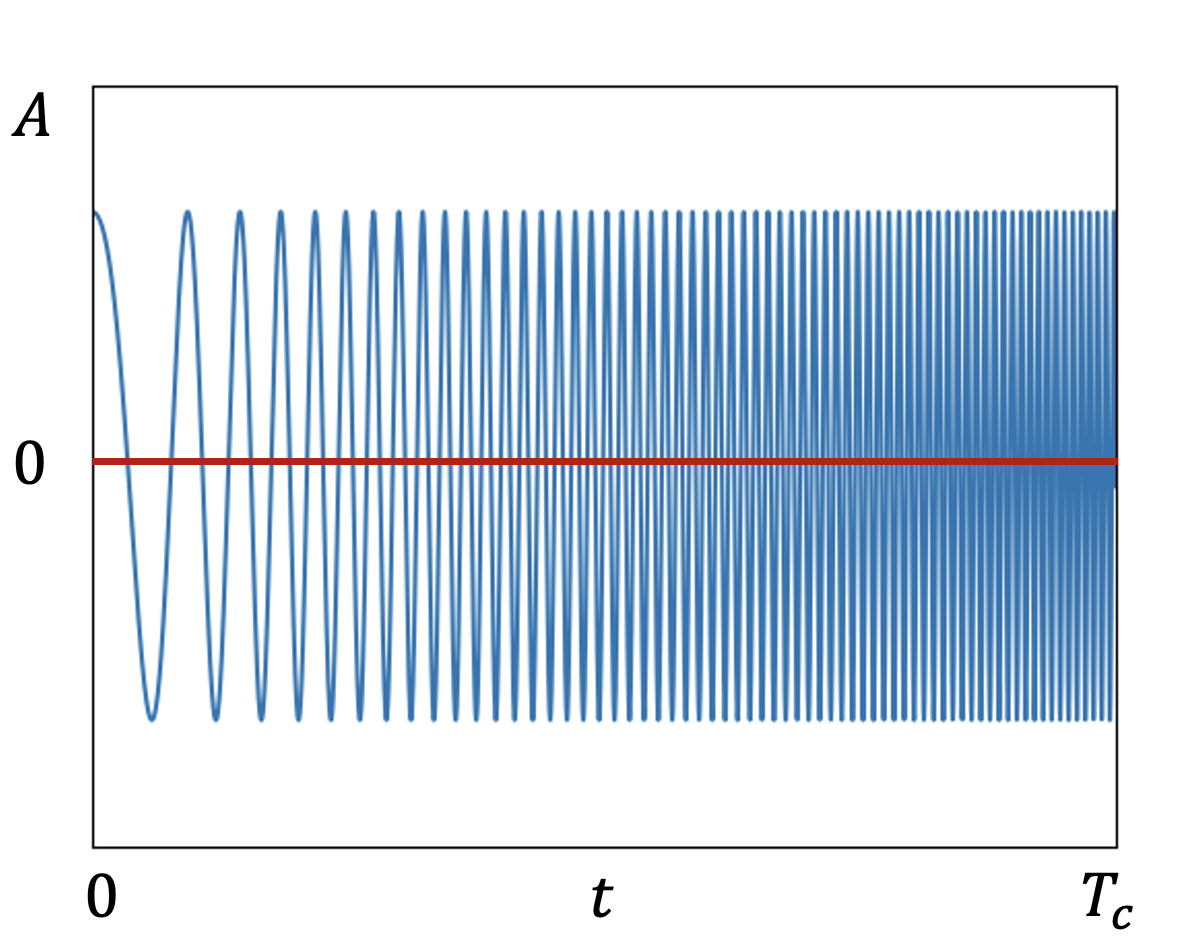
\includegraphics[scale=.3]{figures/FMCW_signal_left.png}}
    \end{subfigure}
    \begin{subfigure}{0.45\textwidth}
        \centering
        \adjustbox{height=5cm}{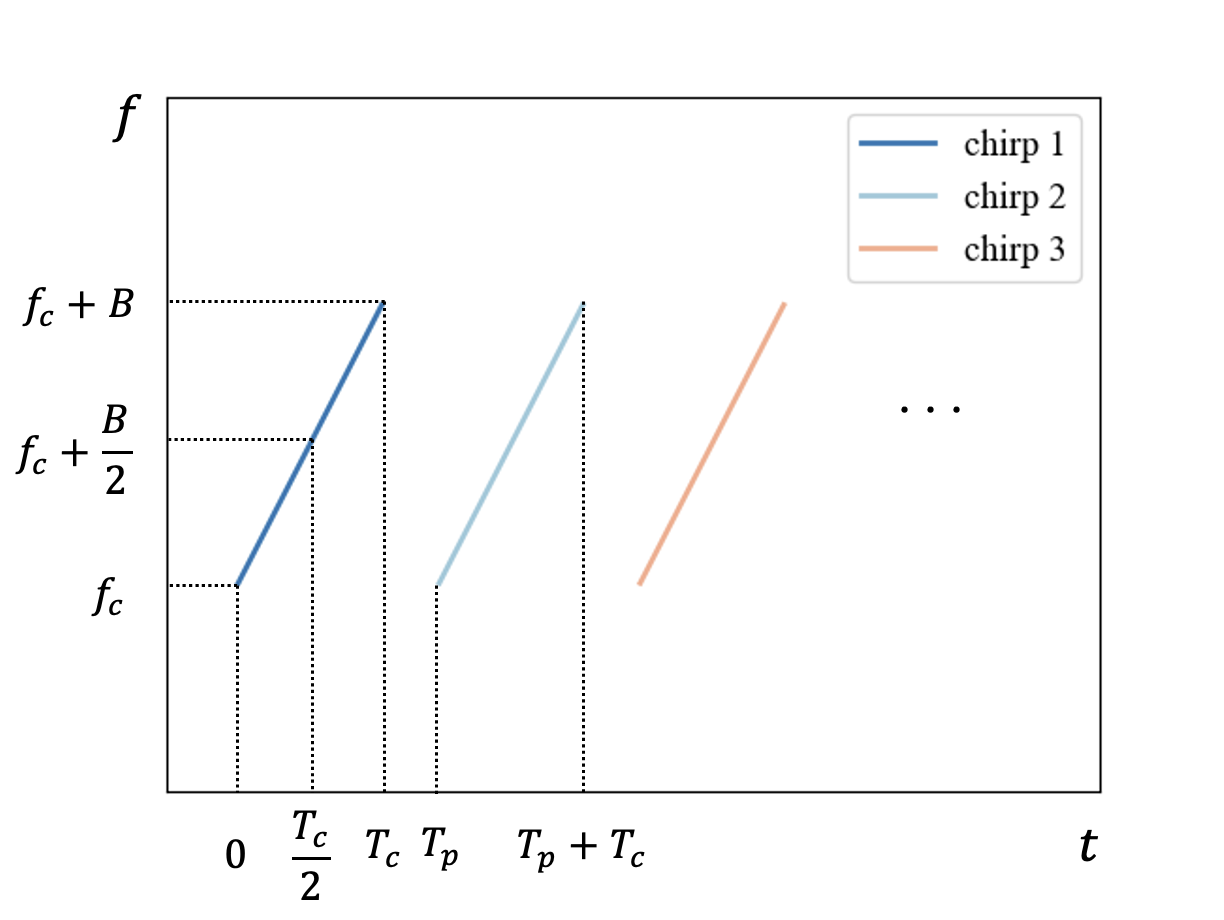
\includegraphics[scale=.3]{figures/FMCW_signal_right.png}}
    \end{subfigure}
    \caption{The amplitude and frequency variation of FMCW radar in time respectively.}
	\label{FMCW_signal}
\end{figure}

Meanwhile, as the reflected signal is captured by the radar, it will be mixed with the transmitted signal in the system to obtain a new signal called \gls{if} signal. The frequency of this \gls{if} signal is theoretically not only depending on the frequency shift $f_r$ caused by the propagation distance but also the Doppler frequency $f_d$, according to \cite{7556357} written as

\begin{equation}
    \centering
    f\textsubscript{IF}\ = f_r - f_d = S \cdot \frac{2r}{c} - \frac{2v}{\lambda},
\end{equation}

but in our case, the Doppler frequency $f_d$ in the beat frequency can be ignored due to the property of the chirp sequence radar, namely

\begin{equation}
    \centering
    f\textsubscript{IF}\ = f_r = S \cdot \frac{2r}{c},
\end{equation}

where the reason will be shown in the next explanation of the chirp sequence radar.

\begin{spacing}{1.5}
\textbf{\large{Chirp sequence radar}}
\end{spacing}

The chirp sequence radar is a \gls{fmcw} radar with the steep frequency ramps \cite{fink_comparison_2015}. The dataset in this paper are collected by a single channel chirp sequence radar \cite{ag_bgt60tr13c_nodate}, which means only a single transmitter and a single receiver are used. In section \ref{dataset recording}, the hardware of the chirp sequence radar will be explained in detail, where there are a single transmitter and three receivers in the radar device. The advantages of using the single channel are following, on one hand, the \gls{mimo} radar will cause a higher cost, hence the single channel radar system reduce the cost to make the localization system cheaper. On the other hand, the signal needs to do the \gls{fft} to convert the signal from time domain into the frequency domain, and the computational complexity will be decreased accordingly.

Due to the difference in the rate of frequency change, the advantage of chirp sequence radar is removing the Doppler frequency part from the \gls{if} signal as mentioned above. The reason is that with the short chirp, i.e. the high value of the slope $S$, the frequency shift $f_r$ will be much larger than the Doppler frequency $f_d$ part. With this property, the radar system will be easy to de-couple the range and velocity estimation, where the range can be calculated by the \gls{if} signal frequency. The estimation of the range is within each chirp which is called the fast time axis, whereas the velocity is calculated by the frequencies of the transmitted and received signals according to the Doppler shift between the chirps which is called the slow time axis, since the time interval between the samples within the chirp is quite short.

\begin{spacing}{1.5}
\textbf{\large{Range-Doppler map}}
\end{spacing}

According to the above, the chirp sequence radar based on the \gls{fmcw} radar can also obtain information about the range and velocity. Meanwhile, there is a corresponding relationship between the range and velocity, which can be drawn through the range-Doppler map. The derivation and visualization process will be shown in detail in section \ref{range-Doppler map visualization}, where the range-Doppler map looks like the one in Figure \ref{an example of the range-Doppler map}.

\begin{figure}
	\centering
	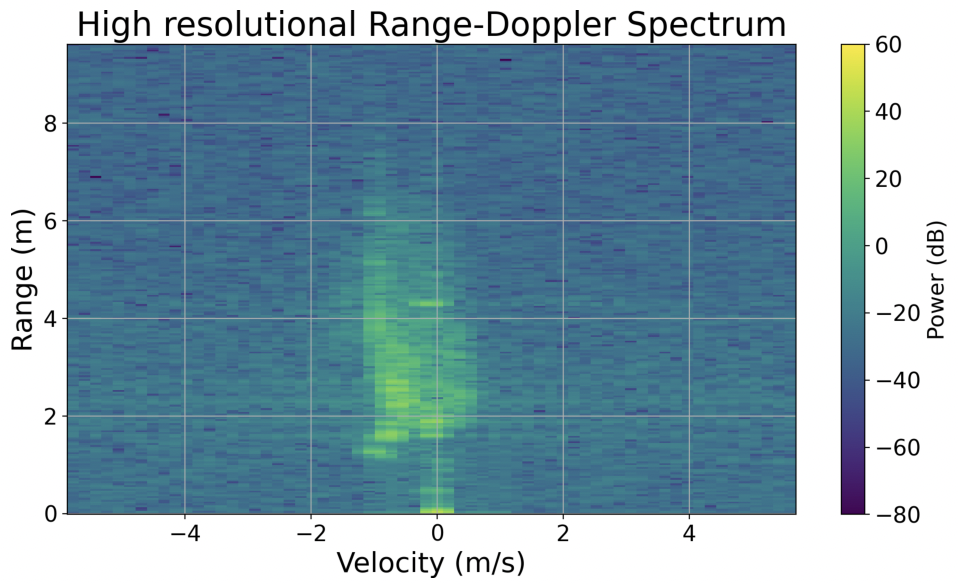
\includegraphics[scale=.6]{thesis/figures/high_res_new.png}
	\caption{An example of the range-Doppler map.}
	\label{an example of the range-Doppler map}
\end{figure}

In the range-Doppler map, the horizontal and vertical axes denote velocity and range respectively. In our dataset, the range is calculated from 0 m to roughly 10 m, and the velocity changes from roughly -5 m/s to 5 m/s. At each point where the range and velocity intersect, the value represents the amplitude about the signal power. When the amplitude is converted to dB unit, the value range is between -80 dB and 60 dB, and the corresponding color in the bar gradually changes from dark to light.


\section{Motivation} \label{motivation}
%The motivation of this thesis and structure of the thesis, show how does the data look like.
As mentioned above, the chirp sequence radar can achieve a larger bandwidth and higher range resolution, but in practical applications, many factors will limit the resolution, such as the hardware of the radar and \gls{cpi}. The carrier frequency and the bandwidth are fixed values in a radar system, since the large bandwidth or high frequency put a higher requirements on the hardware, such as \gls{adc}, antennas and so on, if the cost of the radar system is limited, that is, the frequency or bandwidth are limited, both range and velocity resolutions are influenced. The carrier frequency used by the radar system is affected by many other factors as well, such as regulation. \gls{cpi} refers to the time interval in which the radar continuously observes the targets and performs signal processing. The signal during this time period is coherent, that is, the phase of the signal remains stable and does not change significantly. \gls{cpi} is inversely proportional to the Doppler frequency resolution. In this process, the longer the \gls{cpi}, the more accurate the Doppler frequency resolution can be obtained which leads to a more accurate velocity estimation. However, in many cases, due to the movement of the targets or the ego-motion of the radar itself, the \gls{cpi} is limited, which in turn affects the velocity resolution.

When Figure \ref{an example of the range-Doppler map} is regarded as a high-resolution range-Doppler map, then in reality, the resolution of range and velocity may be only half or even a quarter of that, resulting in a lot of information loss, as shown in Figures \ref{examples of the low resolutional range-Doppler map in different downsampled factor}, where Figure \ref{in halved resolution} shows the effect of the range-Doppler map with the halved resolution, whereas Figure \ref{in quarter resolution} shows a quarter resolutional range-Doppler map.

\begin{figure}
    \centering
    \hspace{-0.4cm}
    \begin{subfigure}{0.5\textwidth}
        \centering
        \adjustbox{height=5cm}{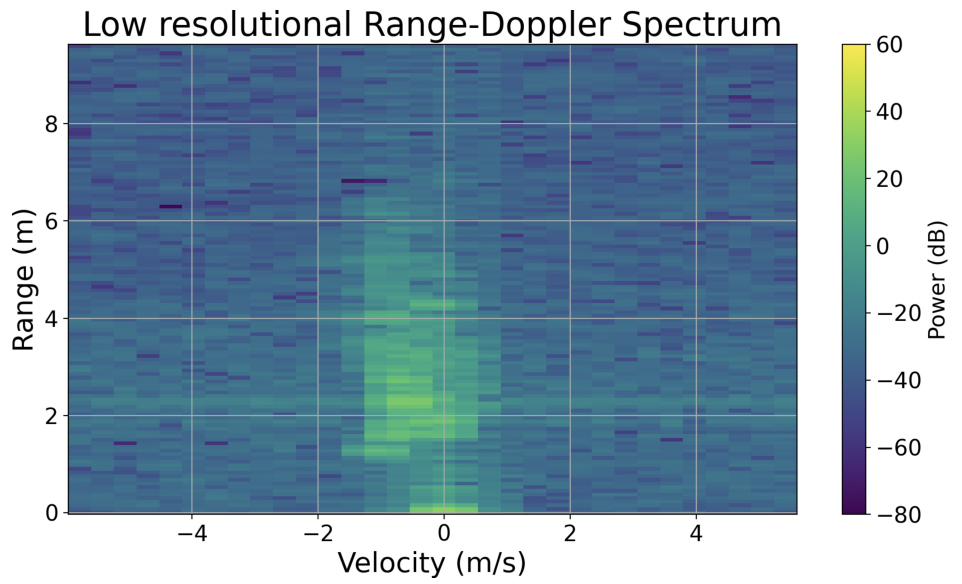
\includegraphics[scale=.24]{thesis/figures/factor_2_new.png}}
        \caption{In halved resolution}
        \label{in halved resolution}
    \end{subfigure}
    \begin{subfigure}{0.5\textwidth}
        \centering
        \adjustbox{height=5cm}{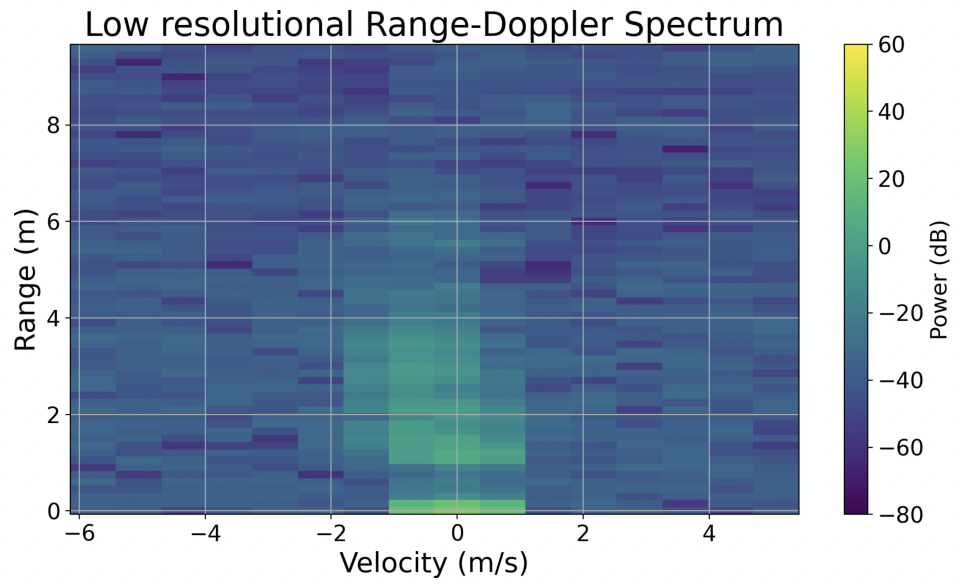
\includegraphics[scale=.24]{thesis/figures/factor_4_new.png}}
        \caption{In quarter resolution}
        \label{in quarter resolution}
    \end{subfigure}
    \caption{Examples of the low-resolution range-Doppler map with different downsampling factor related to the high-resolution range-Doppler map in Figure \ref{an example of the range-Doppler map}.}
	\label{examples of the low resolutional range-Doppler map in different downsampled factor}
\end{figure}

However, high-resolution range-Doppler maps are crucial and have a wide range of applications in areas such as the indoor localization. In order to accurately process and utilize the range-Doppler map, such as \gls{cfar} detection, a high-resolution range-Doppler map is wanted. A traditional, simple and parameter-free method for upsampling is (bi-)linear interpolation. With the development of deep learning, it has shown a strong capability to upsample data to the high resolution. The common structures and models include \gls{cnn}, Encoder-Decoder architecture, Transformer, \gls{cgan} and so on \cite{wang_deep_2021}. Meanwhile, there are also multiple commercial super-resolution solution, such as the super-resolution system in video games provided by NVIDIA \cite{watson2020deep}.

However, the current upsampling approaches are mainly based on images or videos generally, and rarely specifically based on the range-Doppler map of the indoor environment. Compared with the daily images, the range-Doppler map has several significant characteristics. One is that the data in the range-Doppler map have relatively wide dynamic range, especially in the complex environment such as the indoor environment. According to Figure \ref{an example of the range-Doppler map}, the amplitude can be as high as \SI{40}{dB} in places with a closer range, while the noise will be lower than \SI{-60}{dB} in places farther away from the radar. Furthermore, the values in the range-Doppler map are not as visually coherent as those images in the daily life. In addition to the higher values in the parts with closer range, there are usually large differences between even two adjacent points in the surrounding area, which asks for the special requirements on data processing and structure of the model. We would like to process the data so that its dynamic range is relatively smaller. Meanwhile, since each point in the range-Doppler map contains a variety of information such as velocity, range and power, there is a certain correlation between these informations. We hope that the model can learn the connection and relationship between different areas and use deep learning to achieve better upsampling effect than the traditional methods, such as interpolation, and the models commonly used in computer vision.

In addition, another challenge is that our goal is not just based on the closer part, i.e., the area with higher amplitude, but the entire range-Doppler map, including the signals with the lower amplitude. Therefore, in data processing, the purpose of making the range of amplitude smaller not only reduces the dynamic range of the data, but also allows the lower amplitude signals to receive attention.

This thesis will mainly focus on three parts: dataset, models, and loss functions. We will use the radar in the \gls{iss} at the University of Stuttgart to collect the data of the range-Doppler maps and process the dataset. The pipeline will be built to load and process dataset, build and train models, and evaluate them. We will also choose the best data processing methods and the combination of loss functions as well to achieve better upsampling effects for range-Doppler maps.

\section{Structure of the thesis} \label{structure of the thesis}
The thesis will consist of seven chapters. Chapter \ref{introduction} focuses on the introduction of the content in the title and the explanation of some basic concepts, which are completed in section \ref{chirp sequence radar}. Section \ref{motivation} introduced the motivation of the upsampling task based on the range-Doppler map, the challenges, and the ultimate goal of this thesis. Section \ref{structure of the thesis} shows the main structure of the entire thesis and each section. Section \ref{overview of the state of the art} shows the current upsampling approaches in the state of the art, including but not limited to upsampling models for range-Doppler maps.

Chapter \ref{dataset} will focus on the data part. Section \ref{dataset recording} will introduce the information about the data collection, including the hardware of the radar used, the parameters of radar initialization, the settings during the collection process, such as the motion and environmental conditions, and the size of the collected dataset. Moreover, in order to meet our needs, the parameters of the radar as well as the resolution equations will be derived and calculated during the initialization. Section \ref{dataset loading} will show the process of dataset loading, using \gls{tfrecord} files to store data and speed up the loading and training process, and the setting of parameters while creating \gls{tfrecord} files, such as the number of frames, where we use a sliding window for that and the augmentation. In addition, the resampling operation of the data will be demonstrated. Based on the collected high-resolution data, i.e., the ground truth, we create paired low-resolution and high-resolution tuples for training and evaluation by downsampling the high-resolution signals to their respective low-resolution representation. Meanwhile, since the visualization of the range-Doppler map is in the frequency domain, the conversion between the time domain and the frequency domain for the range-Doppler map will also be demonstrated. Section \ref{pre- and post-processing of the model inputs and outputs} will show the processing methods on the models' inputs and outputs. Since the model can only deal with the real value rather than complex value, it could be converted into the concatenation of the real and imaginary part or of the amplitude and phase part, and they can be also normalized or applied logarithm operation to reduce the dynamic range.

Chapter \ref{models} is mainly about the deep learning models used, including a basic \gls{cnn} model, a classical UNet structure and a UNet model that concatenates the decoder part with the encoder part, and two different architectures using Transformer, called \gls{dp}-\gls{tf} Transformer model and \gls{swinir} architecture, respectively in section \ref{dp-tf transformer architecture} and \ref{swinir transformer architecture}. The Transformer architectures have also two types, \gls{dp}-\gls{tf} Transformer block and \gls{swin} Transformer block. Section \ref{comparison between the architecture} will compare the differences between the Transformer architectures and blocks. Section \ref{cgan architecture} will use the above models to design a \gls{cgan} model which contains a generator and introduces a discriminator to implement the adversarial model. Furthermore, in the process of converting data from the time domain to the frequency domain, the range dimension will turn to an odd value, such as from 512 to 257, which will cause problems when the model divide the data into the patches or do the downsampling. Therefore, section \ref{dimension processing layer} will focus on this problem and propose two methods. Additionally, the model must undergo an upsampling layer before the output. There are currently two main methods, which will be introduced in section \ref{upsampling layer}.

Chapter \ref{loss functions} focuses on various loss functions in both training and evaluation phases, and based on the effects of different loss functions, section \ref{combination of the losses} will combine them to complement each other. Chapter \ref{training optimization} will show some methods used in the pipeline to optimize the entire training process, such as using multiple GPUs for distributed training to speed up the training process in section \ref{distributed training}, some settings in the pipeline in section \ref{settings in the pipeline}, and the hyperparameters which can be tuned by the sweep function of the tool WandB shown in section \ref{hyperparameter optimization}.

Finally, Chapter \ref{results} shows the impact of multiple settings, such as different models, processing methods as well as loss functions, on the evaluation loss results, the effect of the super-resolution range-Doppler maps and analyzes them. Chapter \ref{summary and outlook} summarizes the results of the entire thesis and gives the outlook on the further research.

\section{Overview of the state of the art} \label{overview of the state of the art}

%The approaches in the reference papers, and introduce some architectures such as Encoder-Decoder, Transformer and Swin Transformer as well as \gls{cgan} which are normally used in image upsampling.

The state-of-the-art super-resolution methods mainly focus on the supervised learning algorithms \cite{wang_deep_2021}. Currently, the models and structures used in the super-resolution field mainly include \gls{cnn}, residual-based methods, encoder-decoder structure, GAN model, etc \cite{wang_deep_2021}. In addition, Transformer has a strong ability in terms of translation task and wording understanding. The model uses Attention mechanism to understand the association and relationship between different words and phrases, so that it can understand longer sentences than \gls{rnn} \cite{vaswani_attention_2023}. Taking advantage of this feature, the \gls{swin} Transfomer designs a shifted window based on Transformer to divide the data patches and shift windows between them, then different windows can also learn the relationship between each other \cite{liu_swin_2021}.

\begin{spacing}{1.5}
\textbf{\large{Encoder-decoder structure}}
\end{spacing}

The encoder-decoder structure includes two parts. First, it will use encoder to extract features, learn the extracted features, and then use the decoder part to restore the input based on those learned features, so that the model can get the required output. A common structure is called UNet. Olaf et al. apply UNet to segment medical images \cite{ronneberger_u-net_2015}. According to Figure \ref{unet architecture}, the structure of their model is U-shaped. The left side of "U" is the encoder part, that is, the features of the data are extracted and learned, and the right side is the part of the decoder which uses the learned features to restore the data back the original size, while segmenting the objects in the image.

\begin{figure}
	\centering
	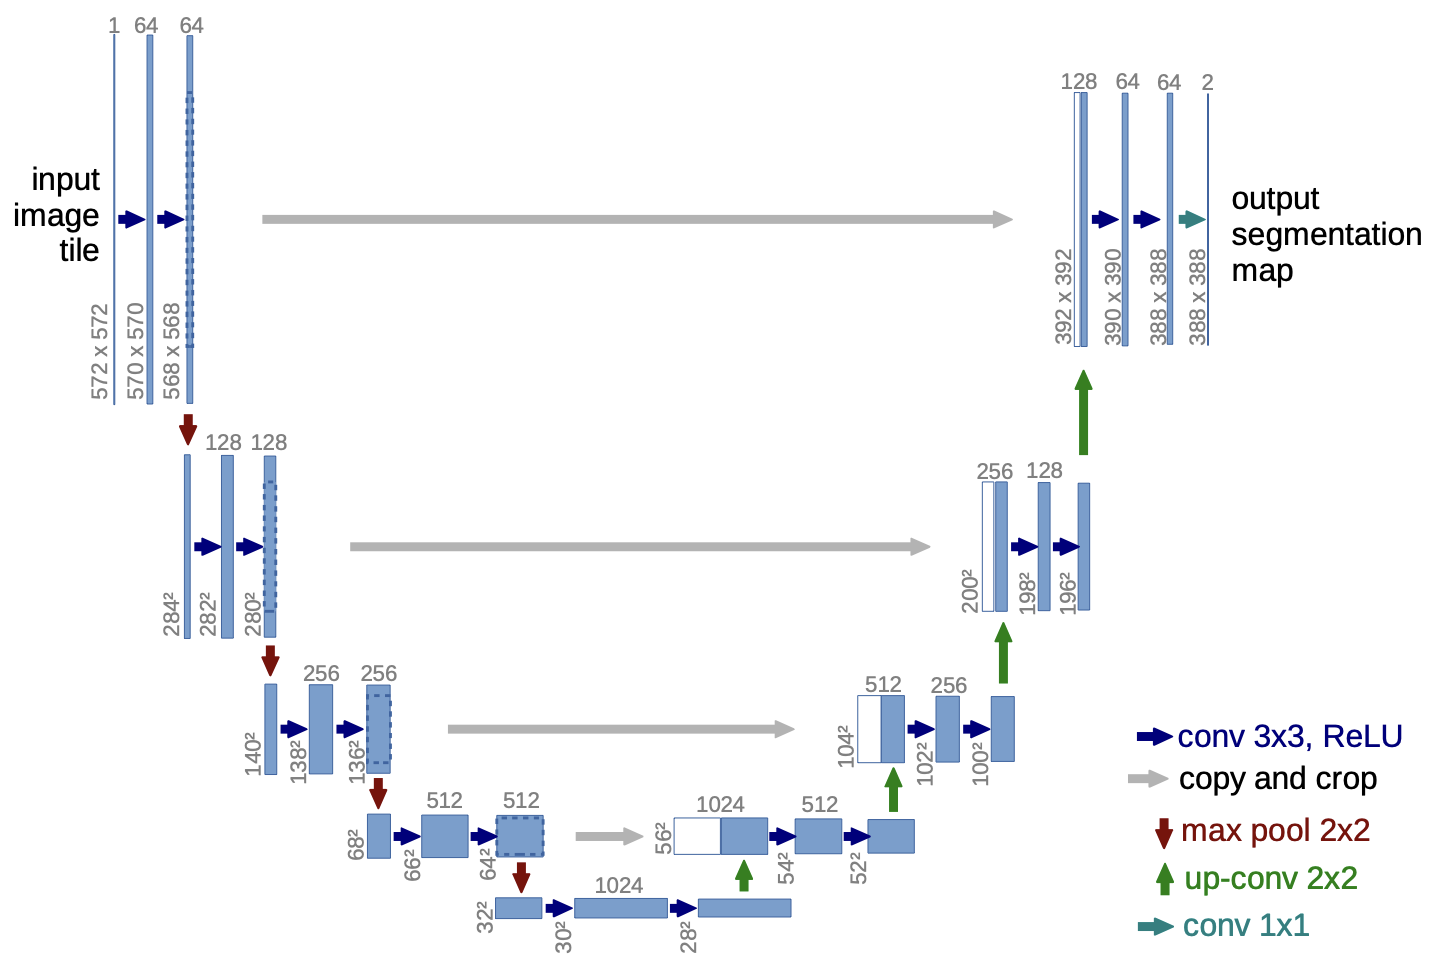
\includegraphics[scale=.5]{figures/unet_paper.png}
	\caption{UNet architecture \cite{ronneberger_u-net_2015}}
	\label{unet architecture}
\end{figure}

In the field of super-resolution data, Akarsh et al. used UNet to upsample the point clouds of mmWave radar \cite{prabhakara_high_2023}. A structure similar to residual path is used in the UNet model, concating the decoder part with the corresponding position of the encoder to alleviate the information loss. The pixel-wise loss and dice loss are combined in the loss function to improve both pixel-wise accuracy and the clarity of the boundary. In the evaluation part, the paper used different environments to test the robustness of the model. Li et al. also applied UNet to the \gls{ra} map collected by \gls{fmcw} radar with \gls{mimo} \cite{li_azimuth_2023}. They have much data processing, inclusive converting the data with the real and imaginary parts, using \gls{fft} to convert the data to a more informative map, and choosing the pixel shuffle method for upsampling.

\begin{spacing}{1.5}
\textbf{\large {Transformer \& Swin Transformer}}
\end{spacing}

In Transformer, the encoder-decoder structure exists as well. There are six identical layers in the encoder part, each layer includes a multi-head attention and a forward propagation sub-layer. According to the attention layer shown in Figure \ref{attention mechanism}, it will calculate the similarity between the query, key and value, thereby obtaining the relationship between different words. In the upsampling task, we will use the self-attention mechanism, that is, query, key and value all come from the same data, thereby obtaining the relationship between the patches. It is on this basis that the \gls{swin} transformer adds shifted windows to achieve that there can be overlapping between windows to improve the uncertainty brought about by fixed split \cite{liu_swin_2021}. Liang et al. proposed the \gls{swinir} architecture based on the \gls{swin} transformer, adding shallow feature extraction and \gls{hq} image restoration \cite{liang_swinir_2021}. The \gls{lq} image will be downsampled once and then passed through multiple \gls{swin} transformers and residual blocks to improve the image resolution.

\begin{figure}
	\centering
	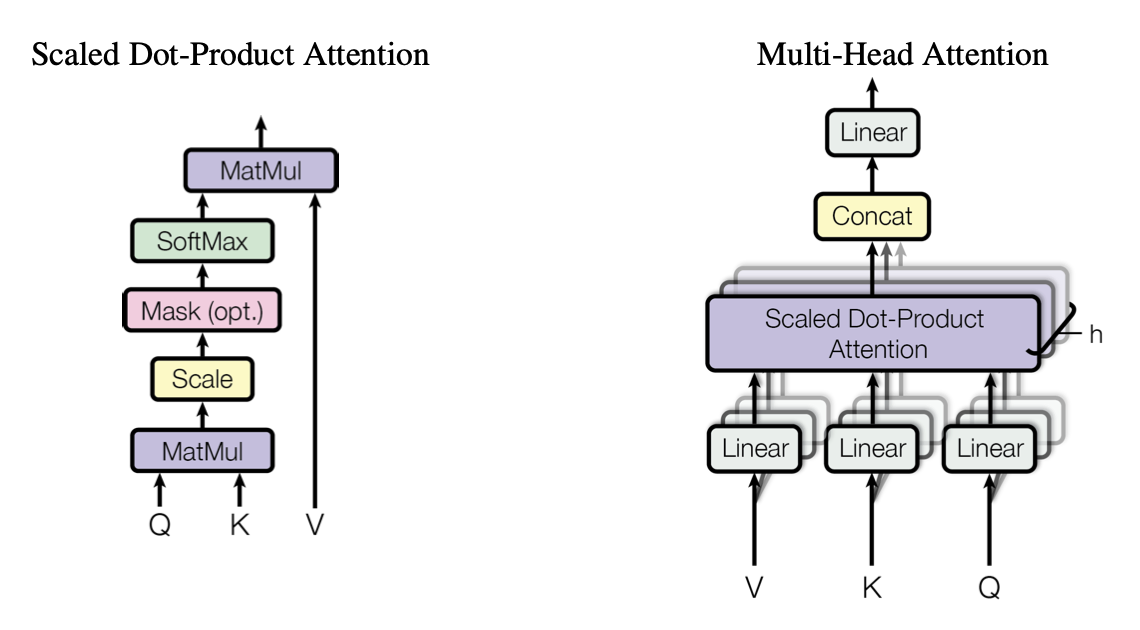
\includegraphics[scale=.65]{figures/attention.png}
	\caption{Attention mechanism \cite{vaswani_attention_2023}}
	\label{attention mechanism}
\end{figure}

The author of \cite{hinderer_blind_2022} proposed a novel approach to separate two signals, which also uses Transformer model, but split the signals along the two coordinates of time and frequency respectively. In addition, due to two signals, it uses a dual-path structure to achieve better distinction between different signal sources. Inspired by this division method, since there are also two obvious dimensions in the range-Doppler map, namely the range and the Doppler effect, we can also try to apply Transformer along these two axes respectively, and the overlapping will exist in this segmentation approach as well.

\begin{spacing}{1.5}
\textbf{\large{GAN \& cGAN models}}
\end{spacing}

The \gls{gan} model also contains two parts, called generator and discriminator. The generator part will extract and learn the data distribution of the input. After generating an output, the discriminator estimates the probability of real and generated samples belonging to the real class. The goal is to make the output of generator as visually close to the ground truth as possible. On the other hand, it is hoped that the discriminator can enhance its discrimination ability and jointly improve the learning ability of the model through adversarial learning between these two parts \cite{goodfellow_generative_2014}.

Based on the \gls{gan} model, Mehdi et al. proposed a conditional version of \gls{gan} model, called \glsfirst{cgan} \cite{mirza_conditional_2014}. \gls{cgan} will feed additional data in the generator and discriminator parts, which is called the condition, as the "y" demonstrated in the Figure \ref{cgan illustrated architecture}. While in our case, the input of the generator is just the low-resolution data as the condition without the noise part. The discriminator will give the probability between the generated super-resolution and real high-resolution range-Doppler maps based on the conditional low-resolution range-Doppler map, which is well shown in Figure \ref{cgan architecture without noise for the generator}.

\begin{figure}
	\centering
	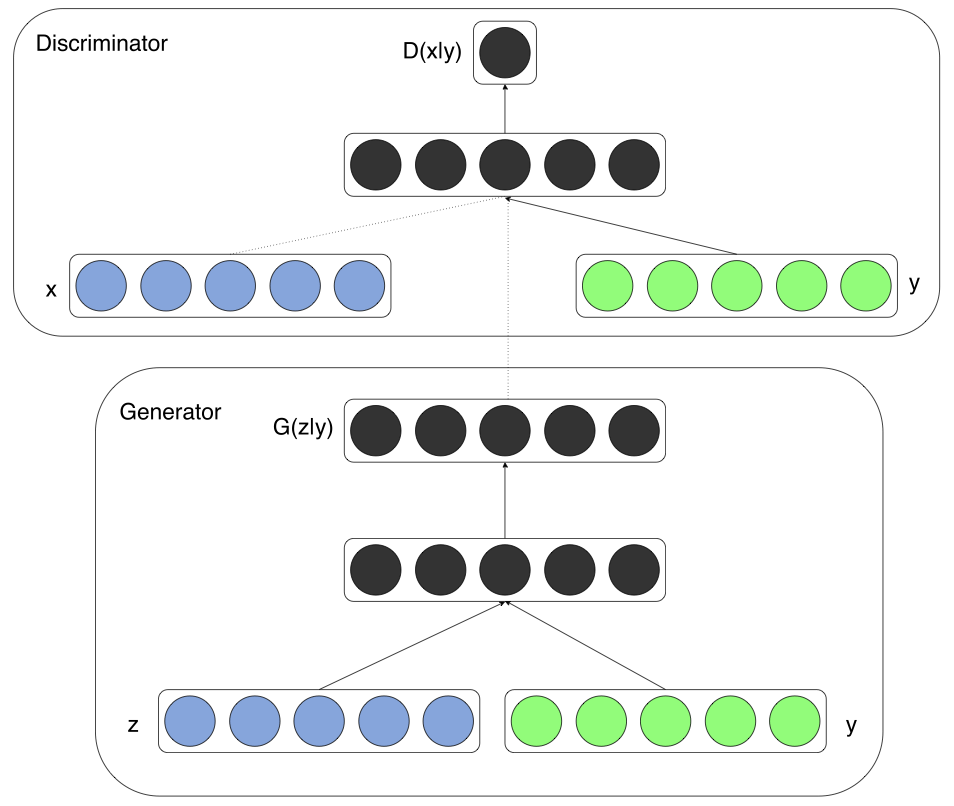
\includegraphics[scale=.65]{figures/cgan_paper.png}
	\caption{cGAN architecture, where x is the ground truth or the generated output, z represents the noise and y is the condition of the model \cite{mirza_conditional_2014}.}
	\label{cgan illustrated architecture}
\end{figure}

\begin{figure}
	\centering
	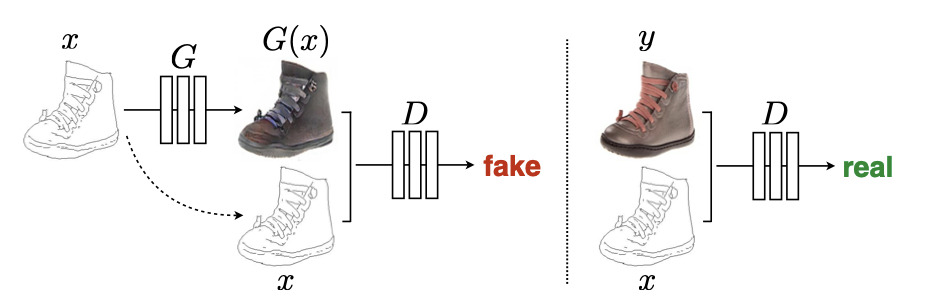
\includegraphics[scale=.8]{thesis/figures/cgan_pix2pix.png}
	\caption{cGAN architecture without noise input for the generator, where x is the conditional low-resolution data and y is the ground truth \cite{isola_image--image_2018}.}
	\label{cgan architecture without noise for the generator}
\end{figure}

In the field of image super-resolution remedy, Karim et al. used the \gls{gan} model on the data of \gls{fmcw} radar, which was based on the micro-Doppler signature of walking human targets \cite{armanious_adversarial_2019}. The \gls{gan} model consists of two parts: the discriminator and the CasNet generator, where the CasNet generator is a stack of multiple UNet models. The loss function combines the pixel-wise L1 loss and the perceptual loss obtained by the discriminator. Compared with the task in this thesis, the content of our range-Doppler map is more complicated and the dynamic range of the data is more obvious.

With the usage of \gls{cgan}, Kong applied it to the super-resolution of \gls{sar} imagery \cite{kong_dmsc-gan_2023}. The structure of UNet is used in the generator, downsampling is performed through the convolutional layer and upsampling is performed through transposed convolutional layer, and an attention mechanism is performed after each dimension change. Furthermore, multiple losses are combined in the loss function, including \gls{gan} loss, VGG perceptual loss and feature matching loss. Inspiration from this, multiple loss functions can also be combined in our training process to achieve better results. Sherif et al. used the \gls{cmgan} model, combining the Transformer with the GAN structure to learn long-distance dependencies and the convolutional layers to exploit local features, which can tackle a variety of tasks, including super-resolution processing of speech \cite{abdulatif_cmgan_2024}.

Also in the field of super-resolution range-Doppler map, Jeong et al. used the \gls{cgan} architecture, in which the generator was based on the UNet model \cite{jeong_resource-efficient_2023}. In the evaluation, more metrics are used, such as \gls{pmse}, \gls{psnr}, etc. However, since the data was collected mainly in open areas such as the playground, the content in the range-Doppler map is relatively simple. Ledig et al., in their SRGAN model, a GAN for super-resolution image, used a larger resampling rate, namely factor of four, which puts higher requirements on the ability of the model \cite{ledig_photo-realistic_2017}. Meanwhile, they combine perceptual loss, adversarial loss and content loss to prevent the loss of high-frequency information and ensure that the boundaries of objects are clear.
